\documentclass[11pt]{article}
\usepackage{hyperref}
\usepackage{enumerate}
\usepackage{tikz,tikz-cd,tikz-3dplot,pgfplots}
\usepackage{amsmath,amsthm,amssymb,amsfonts,amsthm}
\usepackage{mathrsfs}
\usepackage{bm,bbm}
\usepackage{braket}
\usepackage{slashed}
\usepackage{tensor}
\usepackage{indentfirst}
\usepackage[font=small,labelfont=bf]{caption, subcaption}
\usepackage[a4paper, total={6.5in, 9in}]{geometry}
\usetikzlibrary{decorations.markings,positioning,decorations.pathmorphing}
\allowdisplaybreaks
\pgfplotsset{width=10cm, compat=1.16}
\renewcommand\bra[1]{{\langle{#1}|}}
\renewcommand\ket[1]{{|{#1}\rangle}}
\renewcommand\bfdefault{b}

\newtheorem{theorem}{Theorem}[section]
\newtheorem{lemma}[theorem]{Lemma}
\newtheorem{corollary}{Corollary}[theorem]
\theoremstyle{definition}
\newtheorem{definition}{Definition}[section]
\theoremstyle{remark}
\newtheorem{remark}{Remark}[section]

\DeclareMathOperator{\sech}{sech}
\DeclareMathOperator{\csch}{csch}
\DeclareMathOperator{\arcsec}{arcsec}
\DeclareMathOperator{\arccot}{arccot}
\DeclareMathOperator{\arccsc}{arccsc}
\DeclareMathOperator{\arccosh}{arccosh}
\DeclareMathOperator{\arcsinh}{arcsinh}
\DeclareMathOperator{\arctanh}{arctanh}
\DeclareMathOperator{\arcsech}{arcsech}
\DeclareMathOperator{\arccsch}{arccsch}
\DeclareMathOperator{\arccoth}{arccoth} 

\begin{document}
	\title{In-resonance decay channel detection}
	\author{Seokhyeon Song}
	\maketitle
	
	(Introduction here?)
	
	The exact propagator of a scalar field can be written in a form of
	\[\Delta(p^{2})=\frac{i}{p^{2}-M_{0}^{2}+\Pi(p^{2})},\]
	where the self-energy $\Pi(p^{2})$ contains the sum of 1PI loop integrals.
	Following the ``real on-shell'' renormalisation convention, the propagator is
	\[\Delta(p^{2})=\frac{i}{p^{2}-M^{2}+\Pi(p^{2})-\mathrm{Re}\,\Pi(M^{2})}=\frac{iZ}{p^{2}-M^{2}+iZ\,\mathrm{Im}\,\Pi(p^{2})+O((p^{2}-M^{2})^{2})},\]
	where the real on-shell mass $M$ and the field-strength renormalisation $Z$ satisfy (Particles near threshold ref. here)
	\begin{align*}
		M^{2}&=M_{0}^{2}-\mathrm{Re}\,\Pi(M^{2}),\\
		Z^{-1}&=1+\mathrm{Re}\bigg[\frac{d\Pi(p^{2})}{d(p^{2})}\bigg]_{p^{2}=M^{2}}.
	\end{align*}
	To clearly define the model parameters, we set the counterterms so that $M=M_{0}$ and $Z=1$.
	The imaginary part of the denominator of the propagator is related to the particle's total decay width $\Gamma$, where
	\[M\Gamma=Z\,\mathrm{Im}\,\Pi(M^{2}).\]
	Because of unitarity, this definition of decay width coincides with the definition given by the scattering amplitude with one initial state. (More rigorous statement needed. Actually only well-defined in NWA?)
	
	One of the alternative definition uses the complex pole mass $\tilde{M}_{p}$, where the propagator diverges at $p^{2}=\tilde{M}_{p}^{2}$.
	In this framework, the real particle mass $M_{p}$ and the width $\Gamma_{p}$ can be read,
	\[\tilde{M}_{p}=M_{p}-\frac{i}{2}\Gamma_{p}.\]
	This definition seems to be mathematically more concise, but there are subtleties.
	In terms of complex plane of $p^{2}$, the physical Riemann sheet consists of the positive-imaginary half plane and its Schwarz reflection.
	In this sheet, the propagator has no pole.
	In order to get a pole, we have to perform analytic continuation across a branch cut starting from $p^{2}=M_{\mathrm{th}}^{2}$, where the ``threshold invariant mass" $M_{\mathrm{th}}$ is a sum of the masses of decay products.
	If there are more than one available decay channels, then there can be more than one secondary Riemann sheets, each contains complex pole.
	
	If all the threshold invariant masses are sufficiently out off the resonance peak, we can analytically continue the Riemann sheet through the branch near the peak and obtain the complex pole, which agrees well with the real on-shell mass and width.
	The reason is that because the self energy $\Pi(p^{2})$ is an analytic function of $p^{2}$ except on the poles and branch singularities, we may linearly approximate
	\[p^{2}-M_{0}^{2}+\Pi(p^{2})\simeq Z_{p}^{-1}(p^{2}-\tilde{M}_{p}^{2})\]
	near the peak, where $Z_{p}^{-1}$ is the residue of propagator on the pole $p^{2}=\tilde{M}_{p}^{2}$.
	Then
	\[\Delta(p^{2})\simeq\frac{iZ_{p}}{p^{2}-\tilde{M}_{p}^{2}}=\frac{iZ_{p}}{p^{2}-(M_{p}^{2}-\frac{\Gamma_{p}^{2}}{4})+iM_{p}\Gamma_{p}},\]
	suggesting Breit-Wigner distribution.
	The analytic behavior of the propagator also can be seen in Fig. \ref{fig:pole_structure}.
	Typically, decay width of a particle is way smaller than a mass, so we can neglect the $\Gamma_{p}^{2}$ term.
	
	However, if there is an ``in-resonance" decay channel whose threshold invariant mass lies inside the peak, then there exists a branch singularity inside the peak on the real axis, hence such linear approximation is invalid.
	In this case, depending on the point of view, one can say that more than one pole is involving in the resonance, or that no pole explains the resonance well enough.
	Even in this case, the real on-shell definition serves as a definition of the unique mass and width, therefore, the mass and width from now on will only mean the real on-shell values.
	
	\begin{figure}
		\centering
		\begin{subfigure}[b]{0.4\textwidth}
			\centering
			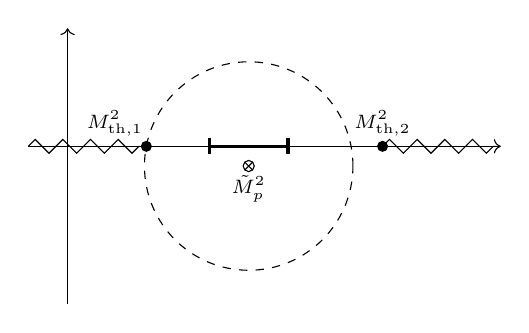
\begin{tikzpicture}
				\draw[->] (-0.5,0) -- (5.5,0);
				\draw[->] (0,-2) -- (0,1.5);
				\draw[decorate,decoration=zigzag] (-0.5,0) -- (1,0);
				\draw[decorate,decoration=zigzag] (4,0) -- (5.5,0);
				\fill (1,0) circle[radius=2pt];
				\fill (4,0) circle[radius=2pt];
				\draw[dashed] (2.3,-0.25) circle[radius=sqrt(1.7525)];
				\draw[very thick] (1.8,0) -- (2.8,0);
				\draw[very thick] (1.8,0.1) -- (1.8,-0.1);
				\draw[very thick] (2.8,0.1) -- (2.8,-0.1);
				\draw (2.25,-0.2) -- (2.35,-0.3);
				\draw (2.25,-0.3) -- (2.35,-0.2);
				\draw (2.3, -0.25) circle[radius=sqrt(2)*0.05];
				\node at (2.3,-0.25) [below]{$\scriptstyle\tilde{M}_{p}^{2}$};
				\node at (0.6,0) [above]{$\scriptstyle M_{\mathrm{th},1}^{2}$};
				\node at (4,0) [above]{$\scriptstyle M_{\mathrm{th},2}^{2}$};
			\end{tikzpicture}
			\caption{}
			\label{fig:pole_structure:out_peak}
		\end{subfigure}
		\begin{subfigure}[b]{0.3\textwidth}
			\centering
			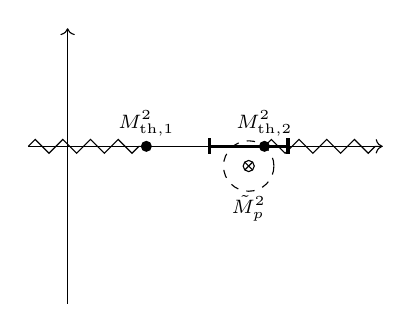
\begin{tikzpicture}
				\draw[->] (-0.5,0) -- (4,0);
				\draw[->] (0,-2) -- (0,1.5);
				\draw[decorate,decoration=zigzag] (-0.5,0) -- (1,0);
				\draw[decorate,decoration=zigzag] (2.5,0) -- (4,0);
				\fill (1,0) circle[radius=2pt];
				\fill (2.5,0) circle[radius=2pt];
				\draw[dashed] (2.3,-0.25) circle[radius=sqrt(0.1025)];
				\draw[very thick] (1.8,0) -- (2.8,0);
				\draw[very thick] (1.8,0.1) -- (1.8,-0.1);
				\draw[very thick] (2.8,0.1) -- (2.8,-0.1);
				\draw (2.25,-0.2) -- (2.35,-0.3);
				\draw (2.25,-0.3) -- (2.35,-0.2);
				\draw (2.3, -0.25) circle[radius=sqrt(2)*0.05];
				\node at (2.3,-0.5) [below]{$\scriptstyle\tilde{M}_{p}^{2}$};
				\node at (1,0) [above]{$\scriptstyle M_{\mathrm{th},1}^{2}$};
				\node at (2.5,0) [above]{$\scriptstyle M_{\mathrm{th},2}^{2}$};
			\end{tikzpicture}
			\caption{}
			\label{fig:pole_structure:in_peak}
		\end{subfigure}
		\captionsetup{width=.9\linewidth}
		\caption{Diagrams demonstrating complex-analytic structure of the propagator $\Delta(p^{2})$, drawn on a complex plane of $p^{2}$. The thick interval indicates the range of resonance peak, and the Riemann sheet is analytically continued through the midpoint of peak. The small circles with cross displays the position of a pole on a secondary Riemann sheet, and the dashed circles means the radius of convergence of the self-energy function $\Pi(p^{2})$, centered on the pole. (a) If every threshold invariant masses are far from the peak, the entirety of peak lies well inside the radius of convergence. Hence, we can take a linear approximation of the self-energy. (b) If there is a threshold invariant mass inside the peak, the self-energy is non-analytic. Thus a linear approximation breaks down.}
		\label{fig:pole_structure}
	\end{figure}
	
	\section{Resonance Shape}
	In the presence of in-resonance decay channel, a shape of resonance peak does not resemble the Breit-Wigner distribution, and a nontrivial momentum dependence of a self-energy becomes important.	
	We will consider one-loop corrections to the scalar particle propagator in terms of renormalisable couplings.
	The momentum dependent contributions in self-energy come from loop diagrams with 2 three-particle vertices.
	For example, consider the following real scalar theory:
	\[\mathcal{L}=\frac{1}{2}\partial_{\mu}X\partial^{\mu}X-\frac{1}{2}M^{2}X^{2}+\mathcal{L}_{\mathrm{int}}.\]
	If a particle $\phi$ which has a mass $m$ interacts with $X$, a process $X\to\phi\bar{\phi}$ has a threshold invariant mass $M_{\mathrm{th}}=2m$.
	Then the self-energy $\Pi(p^{2})$ of $X$ has a branch singularity at $p^{2}=4m^{2}$, but the behaviour of such singularity depends on the spin of $\phi$.
	
	If $\phi$ is a scalar particle, a complex scalar with $\mathcal{L}_{\mathrm{int}}=gX\phi^{\ast}\phi$ for this example, the most singular part of $\Pi(p^{2})$ near threshold is
	\[\Pi(p^{2})=(\mathrm{regular})-\mathrm{sgn}(4m^{2}-p^{2})\frac{g^{2}}{32\pi m}\sqrt{4m^{2}-p^{2}}+O((4m^{2}-p^{2})^{3/2}).\]
	As a function of real variable $p^{2}$, this means that $\Pi(p^{2})$ is continuous but non-differentiable at $p^{2}=4m^{2}$.
	This leads to a typical cusp shape in resonance, as shown in Fig. \ref{fig:resonance_shape:scalar}.
	On the other hand, if $\phi$ is a spinor with $\mathcal{L}_{\mathrm{int}}=gX\bar{\phi}\phi$, then the most singular part of $\Pi(p^{2})$ is
	\[\Pi(p^{2})=(\mathrm{regular})+\mathrm{sgn}(4m^{2}-p^{2})\frac{y^{2}}{16\pi m}(4m^{2}-p^{2})^{3/2}+O((4m^{2}-p^{2})^{5/2}).\]
	This means that $\Pi(p^{2})$ is differentiable at $p^{2}=4m^{2}$.
	This softer singularity suggests that there is no harsh momentum dependence presenting in the resonance shape, as in Fig. \ref{fig:resonance_shape:fermion}.
	If we only look at the imaginary part of the self-energy in $p^{2}>4m^{2}$ region, these spin-dependent results can be reinterpreted as being due to the phase space suppression of decay products.
	
	\begin{figure}[h]
		\centering
		\begin{subfigure}{0.4\textwidth}
			\centering
			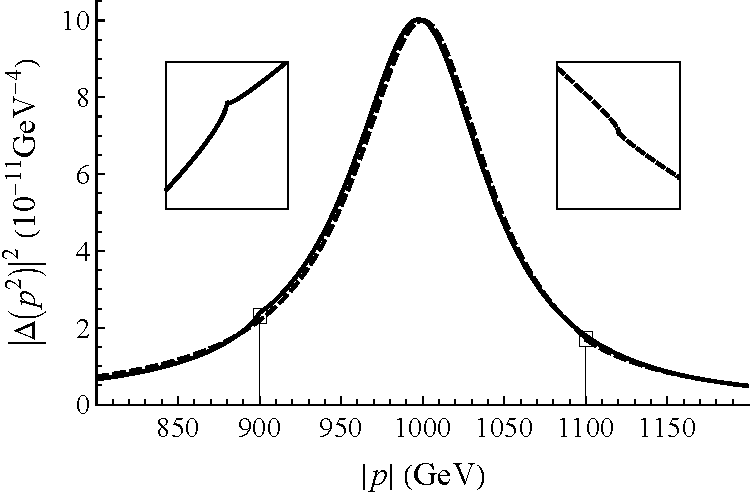
\includegraphics[width=0.9\linewidth]{scalar_resonance_shape.pdf}
			\caption{}
			\label{fig:resonance_shape:scalar}
		\end{subfigure}
		\begin{subfigure}{0.4\textwidth}
			\centering
			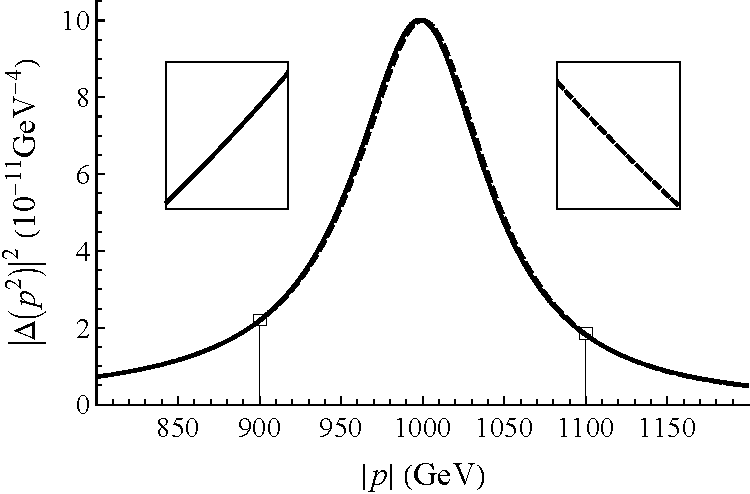
\includegraphics[width=0.9\linewidth]{fermion_resonance_shape.pdf}
			\caption{}
			\label{fig:resonance_shape:fermion}
		\end{subfigure}
		\captionsetup{width=.9\linewidth}
		\caption{Graphs demonstrating resonance shapes of a real scalar particle $X$ up to one-loop order, when the loop particle is (a) a complex scalar and (b) a Dirac fermion. In both cases, the on-shell mass of $X$ is $1\,\mathrm{TeV}$ and the width of $X$ is $100\,\mathrm{GeV}$. For the solid lines, loop particle mass is $450\,\mathrm{GeV}$, so the threshold invariant mass is $900\,\mathrm{GeV}$. The partial width due to the decaying of $X$ into two loop particle is $50\,\mathrm{GeV}$, and the remaining $50\,\mathrm{GeV}$ width is assumed to be due to decay into light particles. For the dashed lines, loop particle mass is $550\,\mathrm{GeV}$, so the threshold invariant mass is $1100\,\mathrm{GeV}$. Here the loop particles do not contribute to the on-shell decay, so all of the width is coming from the light particles. Supplementary graphs show the resonance shapes near the threshold invariant mass.}
		\label{fig:resonance_shape}
	\end{figure}
	
	\section{Toy Statistical Analysis}
	In this paper, we will discuss toy statistical analysis under some simplifying assumptions.
	These assumptions may not hold in real experiment, but statistical analysis of a real experiment requires a lot of information about experimental settings and a detail of new physics model.
	In any case, this simple analysis can be thought of as an approximate analysis of the observability of in-resonance effects.
	We will focus on the dimuon production in accelerators, and ignore other final-state particles.
	We also ignore the angular dependence and only focus on invariant mass $\mu$ of dimuon.
	Integrating out all other degrees of freedom, we left with the differential cross-section $\rho(\mu)=d\sigma/d\mu$.
	
	Suppose that a model predicts a differential cross-section $\rho_{\text{pred}}(\mu;\theta)$, where $\theta$ is a set of model parameters.
	Divide a mass range $M-\Delta M\leq\mu\leq M+\Delta M$ into $N$ bins of equal length, $B_{k}=[\mu_{k-1},\mu_{k}]$ for $k=1,\dots,N$.
	For large enough integrated luminosity $L$, the expected count of samples lying in the $k$th bin is
	\[\bar{n}_{k}(\theta)=L\int_{\mu_{k-1}}^{\mu_{k}}\rho_{\text{pred}}(\mu;\theta)\,d\mu\simeq\frac{2L\Delta M}{N}\rho_{\text{pred}}(\mu_{k};\theta).\]
	The distribution of sample count is Poisson distribution, and it can be approximated by normal distribution if each $\bar{n}_{k}(\theta)$ is sufficiently big.
	In this kind of settings, a good test statistic would be a $\chi^{2}(N)$ statistic, defined by
	\[t(\theta)=\sum_{k=1}^{N}\frac{[n_{k}-\bar{n}_{k}(\theta)]^{2}}{\bar{n}_{k}(\theta)},\]
	where $n_{k}$ is the sample count of each bin measured in the real experiment.
	We may further argue that for $N\gg1$, the value $x:=(t-N)/\sqrt{2N}$ follows the normal distribution.
	Now let $\rho(\mu)$ be the true differential cross-section.
	Then each $n_{k}$ follows the Poisson distribution with the mean $\langle n_{k}\rangle=2L\Delta M\rho(\mu_{k})/N$.
	Then the expected value of $t$ is
	\begin{align*}
		\langle t\rangle(\theta)&=\sum_{k=1}^{N}\frac{1}{\bar{n}_{k}(\theta)}\Big[\langle n_{k}^{2}\rangle-2\bar{n}_{k}(\theta)\langle n_{k}\rangle+\bar{n}_{k}(\theta)^{2}\Big]\\
		&=\sum_{k=1}^{N}\frac{1}{\bar{n}_{k}(\theta)}\Big[\langle n_{k}\rangle^{2}+\langle n_{k}\rangle-2\bar{n}_{k}(\theta)\langle n_{k}\rangle+\bar{n}_{k}(\theta)^{2}\Big]\\
		&=N+\sum_{k=1}^{N}\bigg[\frac{[\langle n_{k}\rangle-\bar{n}_{k}(\theta)]^{2}}{\bar{n}_{k}(\theta)}+\frac{\langle n_{k}\rangle-\bar{n}_{k}(\theta)}{\bar{n}_{k}(\theta)}\bigg].
	\end{align*}
	The second term in the summation is negligible if $\langle n_{k}\rangle-\bar{n}_{k}(\theta)\gg1$, which is likely when $L$ is big enough.
	Then
	\[x(\theta)=\frac{t(\theta)-N}{\sqrt{2N}}\simeq\frac{1}{\sqrt{2N}}\sum_{k=1}^{N}\frac{[\langle n_{k}\rangle-\bar{n}_{k}(\theta)]^{2}}{\bar{n}_{k}(\theta)}.\]
	The best-fit distribution in a specific model is obtained by selecting $\theta$ that minimises $t$.
	
	In the analysis below, we assume that the one-loop calculation for propagators of $X$ is accurate enough to give a true differential cross-section.
	There may be two null hypotheses.
	The first hypothesis $H_{1}$ suggests that the SM background is enough to explain the experiment.
	The second hypothesis, $H_{2}$, agrees that there is a scalar resonance $X$ in dimuon production, but argues that such resonance can be explained by Breit-Wigner distribution.
	If the resonance is narrow enough, the SM background can be considered almost constant within the resonance range.
	We also assume that the SM background is much bigger than the resonance signal, so
	\[\rho_{\text{pred}}(\mu;H_{1})\simeq\rho_{\text{pred}}(M;H_{1})\gg\rho(\mu)-\rho_{\text{pred}}(M;H_{1}).\]
	A scattering amplitude that involves resonant production of dimuon contains the propagator $\Delta(p^{2})$ of $X$.
	If interference is minor, then the discrepancy of differential cross-section from the SM prediction takes the form of
	\[\Delta\rho(\mu)=A(\mu)|\Delta(\mu^{2})|^{2},\]
	where the function $A(\mu)$ can be calculated from the Feynman diagram, excluding the propagator of $X$.
	Again, we assume that $A(\mu)$ is almost constant within the resonance.
	If not, we can always compute $A(\mu)$ from a concrete model.
	Under these assumptions, the test statistic becomes
	\begin{align*}
		x(\theta)&\simeq\frac{1}{\sqrt{2N}}\sum_{k=1}^{N}\frac{[\langle n_{k}\rangle-\bar{n}_{k}(\theta)]^{2}}{\bar{n}_{k}(\theta)}\\
		&\simeq\frac{\sqrt{N}}{\sqrt{8}L\Delta M\rho_{\text{pred}}(M;H_{1})}\sum_{k=1}^{N}[\langle n_{k}\rangle-\bar{n}_{k}(\theta)]^{2}\\
		&\simeq\frac{L}{\sqrt{2N}\rho_{\text{pred}}(M;H_{1})}\int_{M-\Delta M}^{M+\Delta M}[\rho(\mu)-\rho_{\text{pred}}(\mu;\theta)]^{2}d\mu.
	\end{align*}
	Therefore, the required total luminosity to reject the null hypothesis is inversely proportional to square-difference integral of the true distribution and the best-fit distribution.
	In this context, we will calculate the ratio between the integrated luminosity required to reject the hypothesis $H_{1}$ and the one required to reject the hypothesis $H_{2}$.
	This indicates how difficult it is to find the in-resonance decay mode of $X$ compared to discover the scalar resonance itself.
	
	\begin{figure}[h]
		\centering
		\begin{subfigure}{0.4\textwidth}
			\centering
			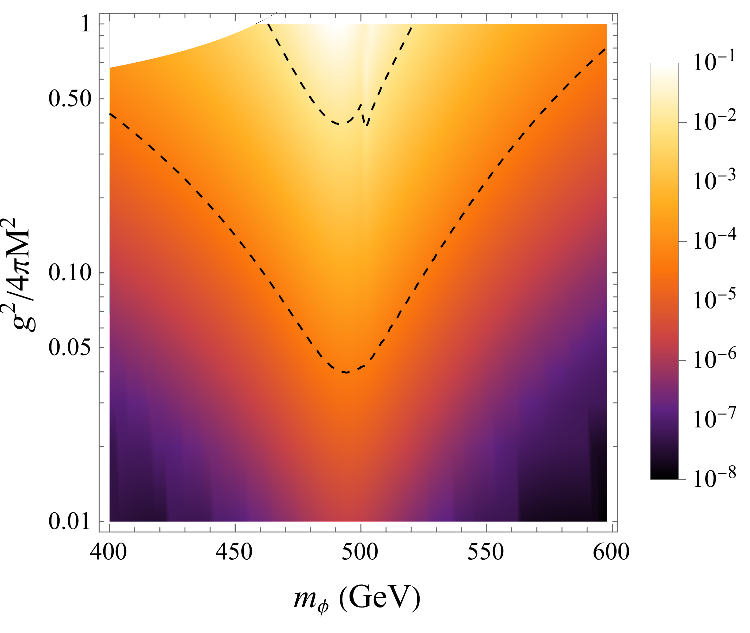
\includegraphics[width=0.9\linewidth]{scalar_0GeV.pdf}
			\caption{}
			\label{fig:luminosity_ratio_sf:scalar}
		\end{subfigure}
		\begin{subfigure}{0.4\textwidth}
			\centering
			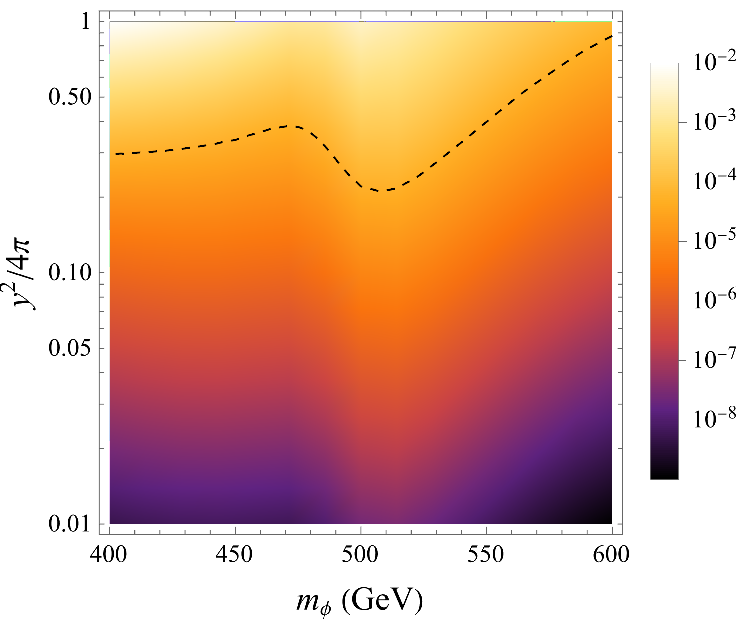
\includegraphics[width=0.9\linewidth]{fermion_0GeV.pdf}
			\caption{}
			\label{fig:luminosity_ratio_sf:fermion}
		\end{subfigure}
		\captionsetup{width=.9\linewidth}
		\caption{Required integrated luminosity ratio of observing in-resonance decay channel, where the loop particle is (a) a complex scalar boson and (b) a Dirac fermion. For example, the value $10^{-2}$ means that $10^{2}$ times of integrated luminosity is needed to confirm the presence of in-resonance decay channel after discovering the scalar resonance. In (a), two dotted lines are the contours having ratio $10^{-2}$ and $10^{-4}$. In (b), a dotted line indicates the ratio value $10^{-4}$, since there is no parameter point making the luminosity ratio greater than $10^{-2}$. In both cases, the mass $M$ of massive real scalar particle is $1\,\mathrm{TeV}$, and the total width of $X$ is $100\,\mathrm{GeV}$. The upper left corner with no data point in graph (a) is the parameter range that the partial width corresponding to $X\to\phi\bar{\phi}$ is greater than the total width, thus is unphysical.}
		\label{fig:luminosity_ratio_sf}
	\end{figure}
	
	\begin{figure}[h]
		\centering
		\begin{subfigure}{0.3\textwidth}
			\centering
			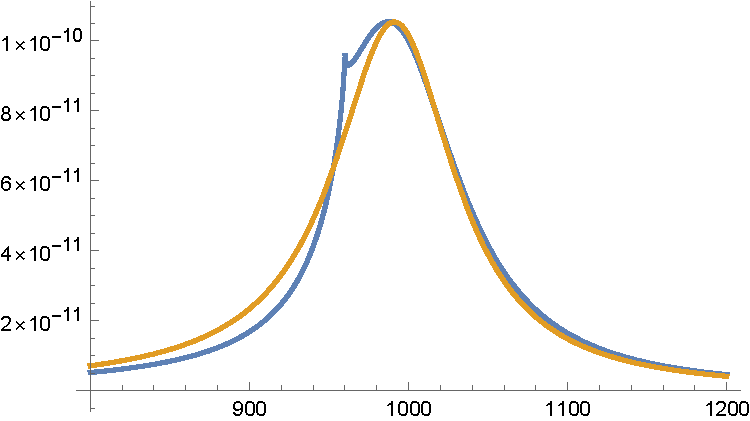
\includegraphics[width=0.9\linewidth]{temp_a.pdf}
			\caption{$m=480\,\mathrm{GeV}$}
			\label{fig:temp:a}
		\end{subfigure}
		\begin{subfigure}{0.3\textwidth}
			\centering
			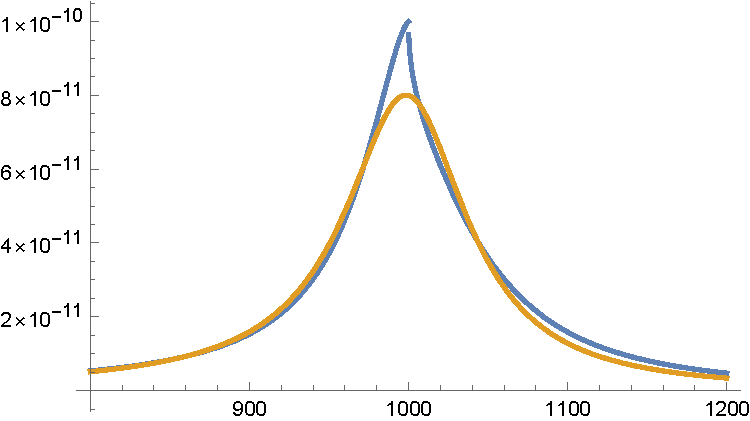
\includegraphics[width=0.9\linewidth]{temp_b.pdf}
			\caption{$m=500\,\mathrm{GeV}$}
			\label{fig:temp:b}
		\end{subfigure}
		\begin{subfigure}{0.3\textwidth}
			\centering
			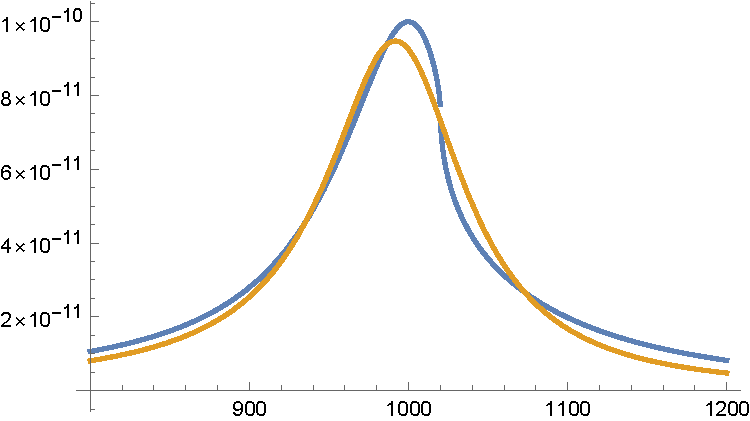
\includegraphics[width=0.9\linewidth]{temp_c.pdf}
			\caption{$m=510\,\mathrm{GeV}$}
			\label{fig:temp:c}
		\end{subfigure}
		\captionsetup{width=.9\linewidth}
		\caption{Temporary plot.}
		\label{fig:temp}
	\end{figure}
	
	As Fig.\ref{fig:luminosity_ratio_sf} shows, it is much harder to discover the in-resonance decay channel into fermions than the in-resonance decay channel into scalar bosons.
	This is consistent with the inability to observe significant changes in the shape of the propagators near the threshold which is shown in Fig.\ref{fig:resonance_shape:fermion}.
	Therefore, in the analysis below, we will focus on the case where the loop particle is a scalar boson.
	
	There is another obstacle in real-world experiments - an uncertainty of measuring dimuon invariant mass, also called smearing.
	This uncertainty is highly dependent on scattering angle, but here we will approximate the effect with simple Gaussian convolution.
	A typical scale of such error is few percent of the momentum, so few tens GeV in this case\footnote{1201.4704 says $\sim10\%$ for $p_{T}\simeq1\,\mathrm{TeV}$. But about $10\,\mathrm{GeV}$ on ILD in best case? 1902.05021}.
	
	\begin{figure}[h]
		\centering
		\begin{subfigure}{0.4\textwidth}
			\centering
			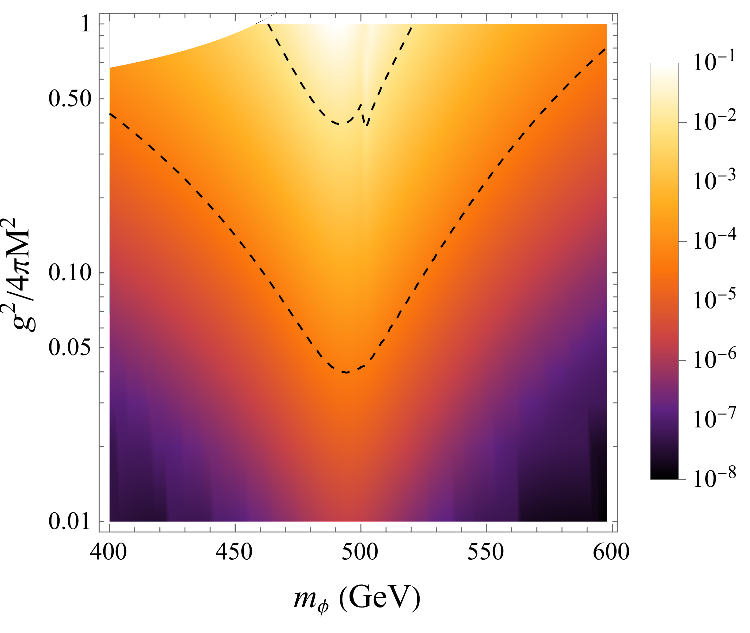
\includegraphics[width=0.9\linewidth]{scalar_0GeV.pdf}
			\caption{}
			\label{fig:luminosity_ratio_scalar:0}
		\end{subfigure}
		\begin{subfigure}{0.4\textwidth}
			\centering
			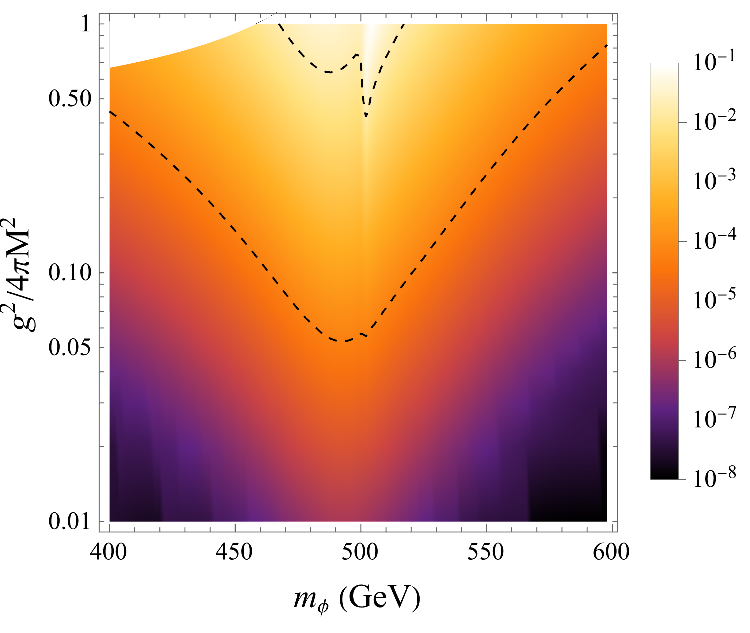
\includegraphics[width=0.9\linewidth]{scalar_10GeV.pdf}
			\caption{}
			\label{fig:luminosity_ratio_scalar:10}
		\end{subfigure}
		\begin{subfigure}{0.4\textwidth}
		\centering
		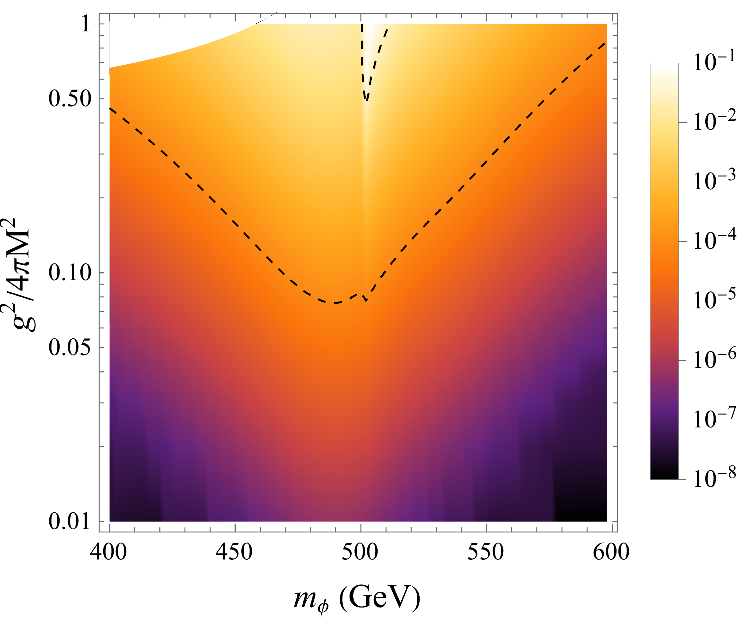
\includegraphics[width=0.9\linewidth]{scalar_20GeV.pdf}
		\caption{}
		\label{fig:luminosity_ratio_scalar:20}
		\end{subfigure}
		\begin{subfigure}{0.4\textwidth}
		\centering
		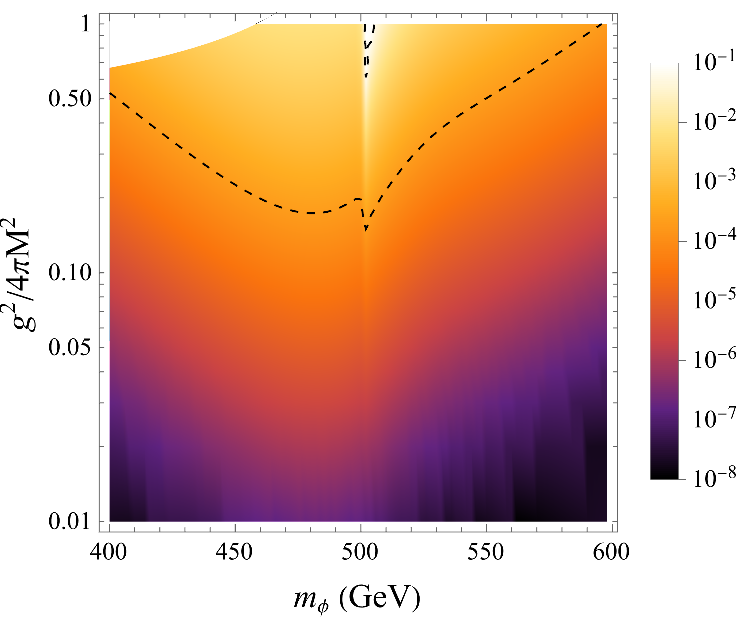
\includegraphics[width=0.9\linewidth]{scalar_50GeV.pdf}
		\caption{}
		\label{fig:luminosity_ratio_scalar:50}
		\end{subfigure}
		\captionsetup{width=.9\linewidth}
		\caption{The luminosity ratio when the smearing is present. The Gaussian uncertainty of the invariant mass is (a) $0\,\mathrm{GeV}$, (b) $10\,\mathrm{GeV}$, (c) $20\,\mathrm{GeV}$, and (d) $50\,\mathrm{GeV}$. The other settings are the same with the one in Fig.\ref{fig:luminosity_ratio_sf:scalar}.}
		\label{fig:luminosity_ratio_scalar}
	\end{figure}
	
	Fig. \ref{fig:luminosity_ratio_scalar} shows the luminosity ratio values while taking smearing into account.
	Clearly smearing worsens the results, especially when the invariant mass uncertainty is in the same order of magnitude with the total width of the particle $X$.
	
	\begin{figure}[h]
		\centering
		\includegraphics[width=0.4\linewidth]{xu_fang.png}
		\caption{Current experimental window for scalar dimuon resonances.}
		\label{fig:CLIC_window}
	\end{figure}
\end{document}